\chapter{Propagating Truncated Differentials}\label{ch:st}
\openepigraph{He that would perfect his work\\must first sharpen his tools.}{Confucius}

\vspace*{-\baselineskip}
\newthought{Synopsis}\hspace{1.5em}
We propose an algorithm for propagating probability-one-subspace trails, and as a generalisation probability-one-truncated differentials, through an iterated function.
Subsequently we discuss two applications.
The first application of this algorithm, is an automated way to prove the resistance of an \SPN/ cipher to subspace trail cryptanalysis.
This is based on the article
\begin{quote}
    \fullfullcite{ToSC:LeaTezWie18}.
\end{quote}
All authors contributed equally.

The second application of our propagation algorithm is about the automation of the key recovery part of a cryptanalytic attack on block ciphers, covered in \cref{ch:key_rec}.

After defining subspace trails and truncated differential attacks, we develop the propagation algorithm for subspace trails.
Additionally to the generic algorithm from~\cite{ToSC:LeaTezWie18}, we here give an improved algorithm for round functions of degree two.
The following sections then describe a method to use this algorithm to prove the absence of subspace trails in an \SPN/ construction.

\section{Introduction}

Truncated differentials have been introduced by Knudsen~\cite{FSE:Knudsen94} more than 20~years ago and since then been used in the analysis of many symmetric primitives, \eg/~\citeonly{C:KnuRobWag99,EC:BloNyb14,ICISSP:Tezcan16,EPRINT:Grassi17}.
Informally, for truncated differentials, instead of trying to understand the exact behaviour of the output difference, one restricts to understand certain patterns that appear in the differences with an unusual high probability.
Surprisingly, even the case of truncated differentials with probability one is not fully understood yet, as this work shows.

Recently, new interest in truncated differentials has been triggered by~\cite{ToSC:GraRecRon16} where the notion of subspace trail cryptanalysis has been defined and used to derive new interesting properties of the \AES/.
As subspace trails are closely related to truncated differentials with probability one, those recent works again highlight that it is important to finally completely understand this topic.

A one round subspace trail can be captured as follows: Given a function $F$ on $n$ bit strings, a subspace trail is specified by two subspaces $U,V \subseteq \F_2^n$, such that any coset of $U$ is mapped to a coset of $V$, that is
\begin{equation*}
    \forall a\in \F_2^n \quad \exists b \in \F_2^n \ \text{such that}\ F(U+a) \subseteq V+b
\end{equation*}
and we denote this by $U \rightarrow V$.

Extending this concept to $r$ rounds of an iterated block cipher with round function $F$, we consider subspace trails given by a tuple of vector spaces $(U_0, \ldots, U_r)$ such that for all $i$ we have
\begin{equation*}
    U_i \rightarrow U_{i+1}.
\end{equation*}

The important question, both for the design as well as for the analysis of block ciphers, is how to identify the most powerful subspace trails, where most powerful basically corresponds to covering as many rounds as possible.
In the case of truncated differentials, several heuristics have been used to solve this problem so far.
For \SPN/ ciphers, where each round function consists of a layer of parallel S-boxes followed by a linear mapping, the two most common ones are to ignore the details of the S-box and to restrict to the cases where $U_0$ only activates one S-box.
While intuitively this approach seems to cover the best subspace trails, it seems hard to exclude the existence of better subspace trails outside those special cases.
Indeed, to underline that the heuristic of activating a single S-box is not sufficient in general we provide several examples (see \cref{st:sec:examples}) where the best subspace trails actually activate more than one S-box.

For the designers of block ciphers it would be very convenient to exclude the existence of subspace trails without making any restrictions and thus to avoid having to base the security arguments of a cipher upon heuristics.

For attackers it is interesting to see if attacks could be improved by avoiding those restrictions.
As an example, the subspace trail used in~\cite{EC:GraRecRon17} does not make use of any specific properties of the \AES/ S-box.
Thus, one important question raised is if those results on \AES/ could actually be improved by taking the specific structure of the \AES/ S-box into account.

\newthoughtpar{Our Contribution}
In this work we rigorously analyse subspace trails for \SPN/ ciphers.
As a result of our considerations, we provide efficient and generic algorithms that can be applied to any \SPN/ cipher and compute the longest subspace trails without any heuristics or restrictions.
Thus, we are able to give a solution to \crefName{prob:alg_res_attack} for subspace trails.

As a first step in \cref{sec:st:prelim}, we recall that it is actually possible to efficiently compute the entire subspace trail for any number of rounds efficiently, \emph{given the starting subspace $U_0$}.
Thus, the task of finding the best solution actually boils down to choosing the best starting spaces $U_0$.
However, a priori there is a huge choice of possible starting spaces and it is clearly inefficient to simply try all possible $U_0$.
We thus have to exhibit a way to reduce the choice of $U_0$ to a suitable number in such a way that we are \emph{guaranteed} to not exclude the best choices.
Our consideration here show an interesting difference depending on whether the S-box used in the cipher has linear structures or not.\footnote{%
    We like to note that both situations, that is S-boxes with and without linear structures occur in actual cipher designs.
}
\textcite{LIGHTSEC:MakTez14} already observed an influence of linear structures on truncated differentials, but restricted themselves to linear structures in the coordinate functions of S-boxes.
By considering all linear structures of an S-box, we are able to fully understand its influence on subspace trails.

More precisely, if the S-box used in the cipher does not have any linear structures (see \cref{sec:st:algorithm1}), we can prove that the approach sketched above, that is to ignore the details of the S-box and to only consider the case where $U_0$ activates a single S-box, always results in the strongest subspace trail.
More technically, we show that in this case for any subspace trail the subspaces $U_i$ are without loss of generality direct products of subspaces that are aligned with the S-box layer.
Note that the \AES/ S-box does not have any linear structures.
In particular, this shows that an attacker cannot hope to improve the work of~\cite{EC:GraRecRon17} by taking the details of the \AES/ S-box into account.

In the case when the S-box actually does have linear structures (see \cref{sec:st:algorithm2}), the situation is slightly more complicated and the choice for $U_0$ remains huge.
However, we show that simply switching from the input subspace of the first S-box layer to the output subspace of the first S-box layer results in a simple and efficient workaround.
Here, we can prove that it is sufficient to consider a very limited choice of at most $k2^n$ choices for the output subspace of the first S-box layer, where $k$ is the number of parallel S-boxes and $n$ is the input size of a single S-box.
The price to pay for this switch is that it is in general unclear if any of those trails can actually be extended backwards through the first S-box layer.
However, using this approach we are able to provably bound the longest subspace trail.
More precisely, our bound is either tight (in the case where we can actually extend trails backwards) or off by at most one round (in the case where we cannot).

All our algorithms are efficient for any concrete instance of a block cipher we are aware of.
We run the algorithms on a number of ciphers and report on the results in the respective parts of \cref{sec:st:algorithm1,sec:st:algorithm2}.
Note that while our results will most likely not lead to new attacks on the ciphers we have been investigating, the main point is that we can now provably exclude the existence of such attacks.

We implemented all algorithms in \textsc{c} and \sage/; the \sage/ the source code is listed in
\cite[Appendix~A]{ToSC:LeaTezWie18}%
%\cref{st:app:impl}
.

\newthoughtpar{Related Work}
Besides the subspace trail on \AES/~\cite{EC:GraRecRon17}, subspace trail cryptanalysis has been applied to \textsc{Prince} in~\cite{INDOCRYPT:GraRec16}.
A paper that is technically related, but focuses on invariant subspaces instead of subspace trails is~\cite{EPRINT:LiuRij17}.

\textcite{ToSC:GraRecRon16} noted the strong connection between subspace trails and truncated differentials with probability one.
Actually subspace trails are a special case of the latter.
Truncated differentials are commonly used for impossible differential cryptanalysis, developed by \textcite{AES:deal} and \citeauthor{EC:BihBirSha99,FSE:BihBirSha99}~\citeonly{EC:BihBirSha99,FSE:BihBirSha99}.
Indeed, truncated differentials with probability one, and thus subspace trails as a special case, can be used to construct impossible differentials, \eg/ by looking for two trails that miss in the middle.

Several automatic tools were proposed for finding impossible differentials.
However, none of them is able to \emph{provably} find the best impossible differential efficiently.

The majority of these do not consider S-box details~\citeonly{INDOCRYPT:KHSLL03,EPRINT:LWLG09,INDOCRYPT:WuWan12,ISCI:LLWG14,EC:SLGRL16,IET-IFS/CJZCZ17}.
Only few attempts were done to understand the influence of the S-box layer.
\textcite{DCC:WanJin17} improve on~\cite{EC:SLGRL16} by analysing this influence in the case of the \AES/.
An attempt to partially cover the S-box influence is the notion of undisturbed bits, developed in the context of probability one truncated differentials~\cite{CAM:Tezcan14}.
\textcite{LIGHTSEC:MakTez14} started to describe undisturbed bits with linear structures of coordinate functions of S-boxes.
Exploiting these bits results in the best known impossible differentials for some block ciphers~\citeonly{CAM:Tezcan14,SIN:TezTasDem14,ICISSP:Tezcan16}.

\textcite{C:DerFou16} and \textcite{EC:SasTod17} tackle the influence of an S-box without restricting to a special one.
The first develop a generic algorithm working on a system of equations which describes the algorithm under scrutiny.
While this in principle allows to handle a very large class of block ciphers, it comes at the cost of an increased runtime.
To solve this problematic long runtime, the authors revert to handling (parts of) the S-box as a black box.
Moreover, the truncated differentials considered are restricted to the case where state bits may be active or passive, while more general subspaces are not handled.
The second use a different approach, namely mixed integer linear programming (MILP).
Due to size constraints, the MILP model is not able to handle 8-bit S-boxes and also block sizes of 256~or~512~bits seem to be out of reach with this technique.
Additionally, the authors did not consider all possible starting differences, but focused on activating only single S-boxes.

\section{Subspace Trails and Truncated Differentials}\label{sec:st:prelim}

Here, we continue our discussion started in \cref{sec:prelim:st}.
Based on \cref{st:def:subspace-trail}, some trivial subspace trails can be observed.
In order to exclude these from our further investigation, we define essential subspace trails.
Furthermore we recapitulate truncated differentials and then show that subspace trails are actually a special case of them.

\subsection{Subspace Trails}

We can identify some trivial subspace trails:
\begin{itemize}
    \item $U = \set{0}$, $V = \set{0}$
    \item pick any $U \subseteq \F_2^n$, $V = \F_2^n$
\end{itemize}
Besides these, if $\propDiff{U}{F}{}{V}$, then for all $U^\prime \subseteq U$ and $V^\prime \supseteq V$ we have $\propDiff{U^\prime}{F}{}{V^\prime}$.
The intuition here is that decreasing $U$ will never result in a bigger $V$ and increasing $V$ does of course also not change the possible output differences in the trail.
This leads to the following definition.

\begin{definition}[Essential Subspace Trail]\label{st:def:essential}
    Let $F : \F_2^n \to \F_2^m$ and $U \subseteq \F_2^n$, $V \subseteq \F_2^m$.
    If $\propDiff{U}{F}{}{V}$ forms a subspace trail, \ie/ $F(U + a) \subseteq V + b$, and if for all subspaces $U^\prime$ and $V^\prime$ of $\F_2^n$ the two properties~\eqref{st:eqn:inc_U} and~\eqref{st:eqn:dec_V} hold, we call $\propDiff{U}{F}{}{V}$ an \emph{essential subspace trail}:
    \begin{alignat}{3}
        \forall U^\prime \supset U &:&\ \nsubspacetrail{U^\prime}{F}{V} \label{st:eqn:inc_U} \\
        \forall V^\prime \subset V &:&\ \nsubspacetrail{U}{F}{V^\prime} \label{st:eqn:dec_V}
    \end{alignat}
\end{definition}
The two properties above ensure that we cannot increase $U$, nor decrease $V$ without destroying the subspace trail property.
Essential subspace trails are clearly the most interesting ones from an attacker perspective.
Another important observation is the following.
\begin{corollary}\label{st:cor:one_dim_trails}
    Let $\propDiff{U_1}{F}{}{U_{2}}$ be a subspace trail through $F$ and
    $V_1 \subseteq U_1$ a subspace contained in $U_1$.
    Then there exists a subspace $V_2 \subseteq U_2$, such that $\propDiff{V_1}{F}{}{V_{2}}$ is also a subspace trail:
    \begin{equation}
    \begin{aligned}
        & U_1 & \propDiff{}{F}{}{}\ &\ U_2 \\
        & \rotatebox[origin=c]{90}{$\subseteq$} & &\ \rotatebox[origin=c]{90}{$\subseteq$} \\
        & V_1 & \propDiff{}{F}{}{}\ &\ V_2
    \end{aligned}
    \end{equation}
\end{corollary}
In other words, it is actually enough to consider one dimensional starting subspaces only, when trying to identify the longest possible subspace trail.
That is, the effect of reducing the initial dimension of the starting subspace can only cause longer subspace trails, not shorter ones.
Thus when we are using this to bound the subspace trail lengths we are potentially only overestimating the length.
%But this overestimation is at most one round.
However, as even in this case the number of starting spaces to consider grows exponentially with the block size, this is still clearly unfeasible for most common block sizes.

We next elaborate on the relation between subspace trails and truncated differentials with probability one.

\subsection{Truncated Differentials}

The following lemma is the key observation that links subspace trails to truncated differentials.
 \begin{lemma}\label{st:lem:st_trunc_diff}
    Given the subspace trail $\propDiff{U}{F}{}{V}$.
    Then
    \begin{equation*}
        \forall u \in U: \Im{\derive{u}{F}} \subseteq V.
    \end{equation*}
    Moreover, for any subspace $U \subset \F_2^n$ it holds that
    \begin{equation*}
        \propDiff{U}{F}{}{\Span{\bigcup_{u \in U} \Im{\derive{u}{F}}}}
    \end{equation*}
\end{lemma}

\cref{fig:st:lemma:image} depicts the intuition of this lemma.
\marginpar{%
    \centering
    %\hspace*{-4.5pt}
    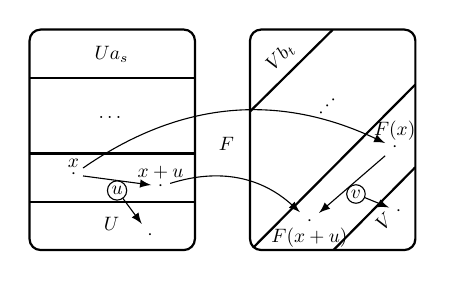
\begin{tikzpicture}[scale=0.7]
        \tikzstyle{every node}=[transform shape];

        \node (left2-space) [draw,rectangle,thick,rounded corners,minimum width=3cm,minimum height=4cm,fill=white] at (1,0) {};
        \draw[thick] (left2-space.west)+(0,1.125cm) -- node[above, yshift=1.5mm] {$\coset{U}{a_s}$} +(3cm,1.125cm);
        \draw[thick] (left2-space.west)+(0,-0.25cm) -- node[above, yshift=5mm] {\dots} +(3cm,-0.25cm);
        \draw[thick] (left2-space.west)+(0,-1.125cm) -- node[below, yshift=-1.5mm] {$U$} +(3cm,-1.125cm);

        \node (right2-space) [draw,rectangle,thick,rounded corners,minimum width=3cm,minimum height=4cm,fill=white] at (5,0) {};
        \draw[thick] (right2-space.north)+(0pt,-0.5pt) -- node[above, yshift=0.5mm, rotate=45] {$\coset{V}{b_t}$} +(-1.5cm,-1.5cm);
        \draw[thick] (right2-space.east)+(-0.5pt,1cm) -- node[above, yshift=10mm, rotate=45] {\dots} +(-3cm+1.25pt,-2cm+1.25pt);
        \draw[thick] (right2-space.east)+(-0.5pt,-5mm) -- node[below, yshift=-0.5mm, rotate=45] {$V$} +(-1.5cm,-2cm);

        \node[xshift=-20pt, yshift=-18pt] (x1) at (left2-space) {$\cdot$};
        \node[above] (x1-label) at (x1) {$x$};

        \node[xshift=32pt, yshift=-4pt] (y1) at (right2-space) {$\cdot$};
        \node[above] (y1-label) at (y1) {$F(x)$};

        \draw[-latex] (x1) to [bend left] node[below,xshift=-2pt,yshift=-10pt] {$F$} (y1);

        \node[xshift=25pt, yshift=-24pt] (x2) at (left2-space) {$\cdot$};
        \node[above] (x2-label) at (x2) {$x+u$};

        \node[xshift=-12pt, yshift=-42pt] (y2) at (right2-space) {$\cdot$};
        \node[below] (y2-label) at (y2) {$F(x+u)$};

        \draw[-latex] (x1) -- node[below,draw,fill=white,inner sep=1pt,circle] (u-label) {$u$} (x2);
        \node[xshift=17pt, yshift=-23pt] at (u-label) (u) {$\cdot$};

        \draw[-latex] (u-label) -- (u);

        \draw[-latex] (x2) to [bend left] (y2);

        \draw[-latex] (y1) -- node[below,xshift=2pt,draw,fill=white,inner sep=1pt,circle] (v-label) {$v$} (y2);
        \node[xshift=22pt, yshift=-9pt] at (v-label) (v) {$\cdot$};

        \draw[-latex] (v-label) -- (v);
    \end{tikzpicture}
    \captionof{figure}{Graphical representation of \cref{st:lem:st_trunc_diff}.}\label{fig:st:lemma:image}
}

\begin{proof}
    Let $u \in U$.
    Because $\propDiff{U}{F}{}{V}$ is a subspace trail for $F$, for any $x \in \F_2^n$: both, $x$ and $x + u$, are in a coset $U + x$ of $U$.
    Due to the subspace trail, they get mapped to a coset of $V$: $F(x), F(x+u) \in V + b$.
    Therefore their sum is again in $V$: $F(x) + F(x + u) \in V$.
\end{proof}

\cref{st:lem:st_trunc_diff} also confirms the intuition that subspace trail attacks and truncated differentials with probability one are closely related.
\textcite{ToSC:GraRecRon16} already discussed this, but we want to state this explicitly:

\begin{corollary}[Link between Subspace Trails and Truncated Differentials]
    Given $\propDiff{U}{F}{}{V}$.
    Then $U$ and $V$ determine a truncated differential with \emph{linear} subspaces that holds with probability one: $\propDiff{\coset{U}{0}}{F}{}{\coset{V}{0}}$.
\end{corollary}

Thus, while subspace trails are included in truncated differentials (as linear subspaces are a special case of affine subspaces), the converse is not true in general.
In other words, using truncated differentials we obtain a bit more information on the actual structure of the investigated function.
This is depicted in the following example.
\begin{example}\label{st:example:present}
We choose a single \present/ S-box, see~\cite{CHES:BKLPPR07}, as $F$ and compute the subspace trail, resp.\ truncated differential, in terms of linear and affine subspaces for the starting difference $\mathtt{0x1}$:
\begin{align*}
    \set{\mathtt{0x0}, \mathtt{0x1}} &\propDiff{}{F}{}{} \set{\mathtt{0x0}, \mathtt{0x3}, \mathtt{0x4}, \mathtt{0x7}, \mathtt{0x9}, \mathtt{0xa}, \mathtt{0xd}, \mathtt{0xe}} \\
    \coset{\set{\mathtt{0x0}}}{\mathtt{0x1}} &\propDiff{}{F}{}{} \coset{\set{\mathtt{0x0}, \mathtt{0x4}, \mathtt{0xa}, \mathtt{0xe}}}{\mathtt{0x9}}
\end{align*}
The affine subspaces we obtain are one dimension smaller than the linear subspaces.
\end{example}
Therefore truncated differentials are rather a generalisation of subspace trails than vice versa.
For the remainder of this work, we focus on the search for subspace trails.

\section{Algorithmic Propagation of Differences}\label{sec:st:compute_trail}

A starting point for finding subspace trails is: Given an initial subspace, how to compute the resulting trail?
One approach is based on \cref{st:lem:st_trunc_diff}.
In order to compute $V$, we have to compute the images of the derivatives of $F$ in direction $U$.
To speed this up, we can exploit two facts.
First, when choosing $x \in_\mathrm{R} \F_2^n$, assuming a random behaviour, it is sufficient to take slightly more than $n$ many $x$ to compute the subspace spanned by the image.
Second, we do not need to compute the image of every element in $U$; instead it is enough to take a basis of $U$, see the following lemma.
\begin{lemma}\label{st:lem:2}
Given $U \subseteq \F_2^n$ and a basis $\Basis{U} = \set{b_1, \ldots, b_k}$ of $U$, then
\begin{equation*}
    \Span{\bigcup_{u \in U} \Im{\derive{u}{F}}} = \Span{\bigcup_{1 \leqslant i \leqslant k} \Im{\derive{b_i}{F}}}\;.
\end{equation*}
\end{lemma}
\begin{proof}
    It is clear that the set on the right side is a subset of the set on the left side of the equation.
    Thus, we are left with showing that the left side is a subset of the right side.
    Moreover, as we consider the linear span on both sides, it suffices to show that any
    \begin{equation*}
        v \in \bigcup_{u \in U} \Im{\derive{u}{F}}
    \end{equation*}
    is contained in
    \begin{equation*}
        \Span{\bigcup_{1 \leqslant i \leqslant k} \Im{\derive{b_i}{F}}}\;.
    \end{equation*}

    We will prove this by induction over the dimension of $U$.
    The case $\dim U =1$ is trivial.
    Now assume that the statement is correct for any $U^\prime$ of dimension smaller than $k$.

    We consider
    \begin{equation*}
        v \in \Im{\derive{u}{F}}
    \end{equation*}
    for $u \in U$.
    That is, there exists an element $x\in \F_2^n$ such that
    \begin{equation*}
        v= \derive{u}{F}(x)= F(x) + F(x + u)\;.
    \end{equation*}
    As the $b_i$ form a basis of $U$, we can express $u$ as a linear combination of the $b_i$, that is
    \begin{equation*}
        u= \sum_{i=1}^k  \lambda_i b_i
    \end{equation*}
    for suitable $\lambda_i \in \F_2$.
    Thus
    \begin{equation*}
        v=F(x) + F(x + \sum_{i=1}^k \lambda_i b_i)\;.
    \end{equation*}
    By defining $x'=x+\lambda_k b_k$ we get
    \begin{align*}
                v= &\ F(x) + F(x + \sum_{i=1}^k \lambda_i b_i) \\
                = &\ F(x^\prime + \lambda_k b_k) +F (x^\prime + \sum_{i=1}^{k-1} \lambda_i b_i) \\
                = &\ F(x^\prime + \lambda_k b_k) + F(x^\prime) + F(x^\prime)+ F(x^\prime + \sum_{i=1}^{k-1} \lambda_i b_i) \\
                = &\ \lambda_k \derive{b_k}{F}(x') + \lambda^\prime \derive{u^\prime}{F}(x')
    \end{align*}
    where
    \begin{equation*}
        \lambda^\prime = \bigvee_{i=1}^{k-1} \lambda_i, \qquad u^\prime = \sum_{i=1}^{k-1} \lambda_i b_i\;.
    \end{equation*}
    Thus
    \begin{equation*}
        v \in \Span{\Im{\derive{b_k}{F}}\cup \Im{\derive{u^\prime}{F}}}\;,
    \end{equation*}
    and the lemma follows by induction as $u'$ is contained in a $(k-1)$ dimensional subspace
    \begin{equation*}
        U^\prime = \Span{b_1,\dots,b_{k-1}}\;.
    \end{equation*}
\end{proof}

Assembling the above observations, we get the recursive \cref{st:alg:compute_trail} to compute the optimal subspace trail for a given starting subspace $U$.
\begin{algorithm}
\caption{Computation of subspace trails}\label{st:alg:compute_trail}
\begin{algorithmic}[1]
    \Require{A nonlinear function $F : \F_2^n \to \F_2^n$, a subspace $U$.}
    \Ensure{A subspace trail $\propDiff{U}{F}{}{\propDiff{\cdots}{F}{}{V}}$.}
    \Statex{}
    \Function{Compute Trail}{$F$, $U$}
    \If{$\dim U = n$}
        \State{}\Return{$U$}
    \EndIf{}
    \State{}$V \leftarrow \emptyset$
    \For{$u_i$ basis vectors of $U$}
        \For{enough $x \in_\mathrm{R} \F_2^n$}\label{st:alg:compute_trail_1line}
            \Let{$V$}{$V \cup \derive{u_i}{F}(x)$}\label{st:alg:compute_trail_2line}
        \EndFor{}
    \EndFor{}
    \State{}$V \leftarrow \Span{V}$
    \State{}\Return{$\propDiff{U}{F}{}{\textsc{Compute Trail}(F, V)}$}
    \EndFunction{}
\end{algorithmic}
\end{algorithm}
% https://math.stackexchange.com/questions/564603/probability-that-a-random-binary-matrix-will-have-full-column-rank
In \cref{st:alg:compute_trail_1line,st:alg:compute_trail_2line} we are sampling random elements of the subspace $V$.
To get the full subspace we are looking for, when computing the span, we have to test enough random~$x$.
Assuming $V$ is a random subspace of $\F_2^n$ and upper bounding its dimension by $n$, we are interested in the probability that $m$~random vectors of length $n$ form a matrix with full rank~$n$.
The probability for the $i$-th vector to be linearly independent of the previous $i-1$ vectors is $1-2^{i-1-m}$.
Thus the probability for all $m$~vectors to be linearly independent is $\prod_{i=0}^{n-1}(1-2^{i-m})$.
This is also known as ${(2^{-m}; 2)}_n$, the 2-Pochhammer symbol or 2-shifted factorial.
Computing ${(2^{-m}; 2)}_n$ shows that it is \enquote{enough} to sample \eg/ $m = n+100$ random $x$ to compute the full subspace $V$ with overwhelming probability.\footnote{%
    With $m = n+100$ we obtain an error probability of $2^{-100}$, and $m=n+20$ results in roughly $2^{-20}$.
}

Note that in the case where $F$ has algebraic degree two, its derivative~$\derive{u_i}{F}$ is linear in all possible directions $u_i$ and thus we can compute $V$ in \cref{st:alg:compute_trail} deterministically.
In this case, similar to the linear layer case below, $V$ has to contain the image of every derivative.
Applying this optimisation yields \cref{st:alg:compute_trail_deg2}.
\begin{algorithm}
\caption{Computation of subspace trails for degree-two functions}\label{st:alg:compute_trail_deg2}
\begin{algorithmic}[1]
    \Require{A nonlinear function $F : \F_2^n \to \F_2^n$ with algebraic degree two, a subspace $U$.}
    \Ensure{A subspace trail $\propDiff{U}{F}{}{\propDiff{\cdots}{F}{}{V}}$.}
    \Statex{}
    \Function{Compute Trail Degree Two}{$F$, $U$}
    \If{$\dim U = n$}
        \State{}\Return{$U$}
    \EndIf{}
    \State{} $\displaystyle V \leftarrow \Span{\bigcup_{u \in \Basis{U}} \Im{\derive{u}{F}}}$
    \State{}\Return{$\propDiff{U}{F}{}{\textsc{Compute Trail Degree Two}(F, V)}$}
    \EndFunction{}
\end{algorithmic}
\end{algorithm}

Unfortunately this still does not reduce the number of possible starting differences.
Thus let us now take a more detailed look at the parts of an \SPN/.
The influence of the linear layer on subspace trails is straightforward.
\begin{proposition}[Subspace trails through linear layers]\label{st:prop:llayer_st}
    Let $L : \F_2^n \to \F_2^n$ be a bijective linear function.
    Then every $U \subseteq \F_2^n$ defines a subspace trail of the form $\propDiff{U}{L}{}{L(U)}$.
    $U$ and $L(U)$ have the same dimension.
    Moreover, any essential subspace trail for $L$ is of this form.
\end{proposition}

\begin{proof}
    Recall that for a subspace trail $\propDiff{U}{L}{}{V}$ it holds that
    \begin{equation*}
        V \supseteq \bigcup_{u \in U} \Im{\derive{u}{L}}.
    \end{equation*}
    For any bijective linear function
    \begin{equation*}
        \Im{\derive{u}{L}} = \set{L(x) + L(x + u)} = \set{L(x) + L(x) + L(u)} = \set{L(u)}.
    \end{equation*}
    As $L$ is bijective, for any pairwise different $u_1$, $u_2 \in U$, $L(u_1)$ and $L(u_2)$ are also different.
    Thus, $V = L(U)$ and $\dim U = \dim V$.
\end{proof}

The S-box layer exhibits a more interesting behaviour.
Here, we need to distinguish between S-boxes without non-trivial linear structures and ones with linear structures.
The first case is covered in \cref{sec:st:algorithm1}, the second in \cref{sec:st:algorithm2}.

Before we study the S-box layer, we will next motivate why the problem of finding the best subspace trail is not as easy as it might seem.


\section{Proving Resistance against Subspace Trail Attacks}
\subsection{Activating Only Single S-boxes}\label{st:sec:examples}

As mentioned in the introduction, one common heuristic used in finding long truncated differentials, is to activate only a single S-box in the input difference.
Due to the close relation of truncated differentials and subspace trails discussed above it seems natural to use the same heuristic for the latter.
Intuitively it may seem that using starting spaces $U$ that contain non-zero values only for a single S-box performs the best.

In this section we argue that this is not always the best approach.
This is done by considering two examples.
The first one is a toy example based on the \present/ S-box, while the second one is the cryptographic permutation \keccak/-f.

\begin{example}\label{st:ex:motivation}
We choose again the \present/ S-box, $F : \F_2^4 \to \F_2^4$, and a block size of 16~bits, so the S-box layer applies four S-boxes in parallel, $F^4 : \F_2^{16} \to \F_2^{16}$.
The round function $R : \F_2^{16} \to \F_2^{16}$ is then $R(x) \coloneqq L \cdot F^4(x)$, where as the linear layer $L$ we choose $L = L^\prime \cdot B^{-1}$, with $L$, $L^\prime$, and $B$ as given in the margin.
\marginpar{%
    \footnotesize
    \vspace{-15em}
    \begin{equation*}
        \setcounter{MaxMatrixCols}{16}
        L = \begin{psmallmatrix}
            0 & 0 & 0 & 1 & 1 & 0 & 1 & 0 & 0 & 0 & 0 & 1 & 1 & 0 & 1 & 0 \\
            1 & 0 & 1 & 1 & 1 & 0 & 1 & 1 & 1 & 0 & 1 & 1 & 1 & 0 & 1 & 1 \\
            0 & 0 & 0 & 0 & 0 & 0 & 0 & 1 & 1 & 0 & 1 & 0 & 1 & 0 & 1 & 1 \\
            0 & 0 & 0 & 1 & 1 & 0 & 1 & 1 & 1 & 0 & 1 & 0 & 0 & 0 & 0 & 0 \\
            1 & 0 & 1 & 0 & 0 & 0 & 0 & 1 & 1 & 0 & 1 & 1 & 1 & 0 & 1 & 1 \\
            0 & 0 & 0 & 1 & 1 & 0 & 1 & 1 & 0 & 0 & 0 & 0 & 0 & 0 & 0 & 1 \\
            0 & 0 & 0 & 1 & 0 & 0 & 0 & 1 & 1 & 0 & 1 & 0 & 1 & 0 & 1 & 0 \\
            0 & 0 & 1 & 1 & 1 & 0 & 1 & 1 & 0 & 0 & 0 & 0 & 1 & 0 & 1 & 0 \\
            1 & 1 & 1 & 0 & 0 & 0 & 0 & 0 & 1 & 0 & 1 & 1 & 0 & 0 & 0 & 1 \\
            1 & 0 & 1 & 1 & 0 & 0 & 1 & 0 & 1 & 0 & 1 & 0 & 1 & 0 & 1 & 0 \\
            1 & 0 & 1 & 1 & 0 & 1 & 0 & 0 & 0 & 0 & 0 & 0 & 0 & 0 & 0 & 0 \\
            0 & 0 & 0 & 0 & 1 & 0 & 1 & 0 & 1 & 0 & 0 & 0 & 0 & 0 & 0 & 0 \\
            1 & 0 & 1 & 1 & 1 & 0 & 1 & 1 & 0 & 1 & 0 & 0 & 1 & 0 & 1 & 1 \\
            0 & 0 & 0 & 0 & 1 & 0 & 1 & 0 & 0 & 0 & 0 & 0 & 1 & 0 & 0 & 0 \\
            1 & 0 & 1 & 1 & 0 & 0 & 0 & 0 & 0 & 0 & 0 & 1 & 1 & 1 & 1 & 0 \\
            0 & 0 & 0 & 1 & 0 & 0 & 0 & 1 & 0 & 0 & 0 & 0 & 1 & 0 & 1 & 0 \\
        \end{psmallmatrix}
    \end{equation*}
    \begin{equation*}
        \setcounter{MaxMatrixCols}{17}
        L^\prime = \begin{psmallmatrix}
            0 & 0 & 0 & 0 & 0 & 0 & 0 & 0 & 0 & & 1 & 1 & 1 & 1 & 1 & 1 & 1 \\
            0 & 0 & 0 & 0 & 0 & 0 & 0 & 0 & 0 & & 1 & 1 & 1 & 0 & 1 & 0 & 1 \\
            0 & 0 & 0 & 0 & 0 & 0 & 0 & 0 & 0 & & 0 & 1 & 0 & 1 & 0 & 0 & 0 \\
            0 & 0 & 0 & 0 & 0 & 0 & 0 & 0 & 0 & & 1 & 0 & 1 & 1 & 0 & 0 & 0 \\
            0 & 0 & 0 & 0 & 0 & 0 & 0 & 0 & 0 & & 0 & 0 & 0 & 0 & 0 & 1 & 0 \\
            0 & 0 & 0 & 0 & 0 & 0 & 0 & 0 & 0 & & 0 & 0 & 1 & 0 & 0 & 0 & 1 \\
            0 & 0 & 0 & 0 & 0 & 0 & 0 & 0 & 0 & & 1 & 1 & 0 & 0 & 1 & 1 & 1 \\
            1 & 0 & 0 & 0 & 0 & 0 & 0 & 0 & 0 & & 1 & 0 & 0 & 1 & 1 & 0 & 1 \\
            0 & 1 & 0 & 0 & 0 & 0 & 0 & 0 & 0 & & 0 & 0 & 1 & 0 & 0 & 1 & 0 \\
            0 & 0 & 1 & 0 & 0 & 0 & 0 & 0 & 0 & & 1 & 1 & 1 & 1 & 1 & 0 & 0 \\
            0 & 0 & 0 & 1 & 0 & 0 & 0 & 0 & 0 & & 0 & 1 & 1 & 0 & 1 & 1 & 0 \\
            0 & 0 & 0 & 0 & 1 & 0 & 0 & 0 & 0 & & 1 & 0 & 0 & 1 & 0 & 0 & 0 \\
            0 & 0 & 0 & 0 & 0 & 1 & 0 & 0 & 0 & & 0 & 1 & 1 & 0 & 0 & 0 & 0 \\
            0 & 0 & 0 & 0 & 0 & 0 & 1 & 0 & 0 & & 0 & 0 & 1 & 1 & 1 & 0 & 1 \\
            0 & 0 & 0 & 0 & 0 & 0 & 0 & 1 & 0 & & 1 & 0 & 1 & 0 & 1 & 1 & 0 \\
            0 & 0 & 0 & 0 & 0 & 0 & 0 & 0 & 1 & & 0 & 0 & 1 & 1 & 0 & 1 & 0 \\
        \end{psmallmatrix}
    \end{equation*}
    \begin{equation*}
        \setcounter{MaxMatrixCols}{17}
        B = \begin{psmallmatrix}
            1 & 0 & 0 & 0 & 0 & 0 & 0 & 0 & 1 & & 1 & 0 & 0 & 1 & 0 & 1 & 0 \\
            0 & 1 & 0 & 0 & 0 & 0 & 0 & 0 & 0 & & 1 & 1 & 1 & 0 & 0 & 0 & 1 \\
            1 & 0 & 0 & 0 & 0 & 0 & 0 & 0 & 0 & & 1 & 0 & 1 & 1 & 0 & 1 & 1 \\
            0 & 0 & 0 & 0 & 0 & 0 & 0 & 0 & 1 & & 1 & 1 & 1 & 1 & 0 & 1 & 1 \\
            0 & 0 & 1 & 0 & 0 & 0 & 0 & 0 & 1 & & 1 & 0 & 1 & 0 & 1 & 0 & 0 \\
            0 & 0 & 0 & 1 & 0 & 0 & 0 & 0 & 0 & & 1 & 0 & 1 & 1 & 1 & 0 & 0 \\
            0 & 0 & 1 & 0 & 0 & 0 & 0 & 0 & 0 & & 1 & 0 & 1 & 1 & 0 & 0 & 0 \\
            0 & 0 & 0 & 0 & 0 & 0 & 0 & 0 & 1 & & 1 & 0 & 1 & 0 & 0 & 1 & 0 \\
            0 & 0 & 0 & 0 & 1 & 0 & 0 & 0 & 1 & & 1 & 0 & 0 & 0 & 1 & 0 & 0 \\
            0 & 0 & 0 & 0 & 0 & 1 & 0 & 0 & 0 & & 0 & 0 & 0 & 0 & 0 & 1 & 1 \\
            0 & 0 & 0 & 0 & 1 & 0 & 0 & 0 & 0 & & 0 & 1 & 1 & 1 & 0 & 0 & 1 \\
            0 & 0 & 0 & 0 & 0 & 0 & 0 & 0 & 1 & & 0 & 1 & 1 & 1 & 0 & 1 & 1 \\
            0 & 0 & 0 & 0 & 0 & 0 & 1 & 0 & 1 & & 0 & 0 & 1 & 0 & 0 & 0 & 1 \\
            0 & 0 & 0 & 0 & 0 & 0 & 0 & 1 & 0 & & 0 & 1 & 1 & 0 & 1 & 0 & 0 \\
            0 & 0 & 0 & 0 & 0 & 0 & 1 & 0 & 0 & & 0 & 1 & 0 & 0 & 0 & 1 & 0 \\
            0 & 0 & 0 & 0 & 0 & 0 & 0 & 0 & 1 & & 0 & 1 & 1 & 0 & 1 & 0 & 0 \\
        \end{psmallmatrix}
    \end{equation*}
}

Let us first observe which subspace trails this round function exhibits.
Almost all subspace trails starting with only one active S-box are of the form
\begin{equation*}
    \mathrm{dim}\ 1 \rightrightarrows \mathrm{dim}\ 4 \rightrightarrows \mathrm{dim}\ 16.
\end{equation*}
Thus reaching the full dimension after two rounds.
In contrast to this, the subspace trail with a $\mathtt{0x1}$ difference on every S-box input, more precisely the starting subspace is $\set{\mathtt{0x0000}, \mathtt{0x1111}}$ -- which is one dimensional but activates all four S-boxes in the beginning, has the following form:
\begin{equation}\label{st:eqn:example1}
    \mathtt{0x1111} :\quad \mathrm{dim} 1 \rightrightarrows \mathrm{dim} 9 \rightrightarrows \mathrm{dim} 11 \rightrightarrows \mathrm{dim} 16,
\end{equation}
effectively lasting for a full additional round.
This is of course due to the special structure of the linear layer.
The left part of the chosen basis $B$ consists of exactly the vectors spanning the space of dimension nine after the first round.
In combination with the given $L^\prime$, all these vectors are then mapped to only activating the rightmost three S-boxes (with a $\mathtt{0x1}$ difference on the third S-box), leaving the last S-box passive.

Still, there are four subspace trails, with only one active S-box, that also reach three rounds:
\begin{align*}
    \mathtt{0x1000} &:\quad \mathrm{dim}\ 1 \rightrightarrows \mathrm{dim}\ 3 \rightrightarrows \mathrm{dim}\ 14 \rightrightarrows \mathrm{dim}\ 16 \\
    \mathtt{0x0001} &:\quad \mathrm{dim}\ 1 \rightrightarrows \mathrm{dim}\ 3 \rightrightarrows \mathrm{dim}\ 15 \rightrightarrows \mathrm{dim}\ 16 \\
    \mathtt{0x0f00} &:\quad \mathrm{dim}\ 1 \rightrightarrows \mathrm{dim}\ 3 \rightrightarrows \mathrm{dim}\ 14 \rightrightarrows \mathrm{dim}\ 16 \\
    \mathtt{0x000f} &:\quad \mathrm{dim}\ 1 \rightrightarrows \mathrm{dim}\ 3 \rightrightarrows \mathrm{dim}\ 15 \rightrightarrows \mathrm{dim}\ 16
\end{align*}
But note that all these subspace trails are worse, as the last dimension, before reaching the full dimension, is higher than eleven.
In this example it is thus not the best choice, to activate only one S-box.
Also note that the resulting linear layer $L$ looks sufficiently random, \st/ its hidden structure might be hard to find.
Of course it is very unlikely that such an effect occurs, when the design of the linear layer follows \eg/ the wide trail strategy.
\end{example}

\begin{example}
A real-world example of the above observation is the SHA-3 hash function, more precisely \keccak/-f~\cite{keccak,FIPS:SHA3}.
Starting with any subspace trail of dimension one that has only one active S-box gives us a three round trail with final dimension 1139 in the best case.
But instead starting with an other one dimensional subspace trail with \emph{two} active S-boxes results in a different three round trail that has dimension 949 -- a huge reduction compared to the initial trail.
The exact dimensions are the following:
\begin{align*}
    1\times \mathtt{0x4} &:\quad \mathrm{dim}\ 1 \rightrightarrows \mathrm{dim}\ 3 \rightrightarrows \mathrm{dim}\ 65 \rightrightarrows \mathrm{dim}\            1139 \rightrightarrows \mathrm{dim}\ 1600 \\
    2\times \mathtt{0x4} &:\quad \mathrm{dim}\ 1 \rightrightarrows \mathrm{dim}\ 5 \rightrightarrows \mathrm{dim}\ 49 \rightrightarrows \mathrm{dim}\ \hphantom{0}949 \rightrightarrows \mathrm{dim}\ 1600
\end{align*}
\end{example}

The big advantage of looking only at possible input spaces with one active S-box is the huge reduction in starting points we need to analyse.
But as we have just seen, we cannot rely on these special inputs, when we want to prove the absence of subspace trails.
While we can argue with \cref{st:cor:one_dim_trails} that it is enough to look at trails starting with a one dimensional subspace, we are still facing the problem to cope with exponentially many possible subspace trails.
In the next sections, we develop arguments and algorithms to again reduce this complexity.

\subsection{S-box layers without Linear Structures}\label{sec:st:algorithm1}

The distinction of S-boxes based on their linear structures is based on the following lemma that explains the link.
Recall that $\mathrm{L}_u(F)$ is defined as the set of all $\alpha$ such that for a fixed $ c \in \F_2$
\begin{equation*}
    \iprod{\alpha}{\derive{u}{F}(x)} = c \quad \forall x \in \F_2^n\;.
\end{equation*}

Let us start by considering a single S-box $F:\F_2^n \to \F_2^n$ only.
\begin{lemma}\label{st:lem:vperp_subtrail}
    Given an essential subspace trail $\propDiff{U}{F}{}{V}$.
    Then $V^\perp = \displaystyle\bigcap_{u \in U} \mathrm{L}_{u}(F)$.
\end{lemma}

\begin{proof}
    According to \cref{st:lem:st_trunc_diff} it holds that
    \begin{equation*}
        \forall x \in \F_2^n \ \forall u \in U: \derive{u}{F}(x) \in V\;.
    \end{equation*}
    Now, for an arbitrary element $\alpha \in V^{\perp}$ this implies that
    \begin{equation*}
        \forall x \in \F_2^n \ \forall u \in U: \iprod{\alpha}{\derive{u}{F}(x)} = 0\;.
    \end{equation*}
    Thus
    \begin{equation*}
        V^\perp = \bigcap_{u \in U} \mathrm{L}_{u}(F)
    \end{equation*}
    and, as the trail is essential, the statement follows.
\end{proof}

In particular we have \cref{st:cor:trivial_st} as a direct consequence.
\begin{corollary}\label{st:cor:trivial_st}
    If $F$ has no non-trivial linear structure, then there are only two essential subspace trails: $\propDiff{\set{0}}{}{}{\set{0}}$ and $\propDiff{\F_2^n}{}{}{\F_2^n}$.
\end{corollary}

The most important observation is that, in the case of $F$ without linear structures, a similar observation holds for the entire S-box layer consisting of $k$ parallel S-boxes.
Namely, in this case any essential subspace trail is \emph{the direct product of subspace trails of the single S-box}.
This implies with the \cref{st:cor:trivial_st} that any essential subspace trail through an S-box layer can simply be characterised by active and passive S-boxes.
The following proposition covers exactly this.
\begin{proposition}[Subspace trails through S-box layers]\label{st:prop:no_ls}
    Let $F^k$ be an S-box layer, and $\propDiff{U}{F^k}{}{V}$ an essential subspace trail.
    If $F$ has no non-trivial linear structures, then
    \begin{equation*}
        U = V = U_1 \times \cdots \times U_k
    \end{equation*}
    where for $1 \leqslant i \leqslant k$ it holds that $U_i \in \{ \{0\}, \F_2^n\}$.
\end{proposition}
\begin{proof}
    Let $\propDiff{U}{F^k}{}{V}$ be essential.
    Then $\forall \alpha = (\alpha_1, \ldots, \alpha_k) \in V^\perp$ the following holds
    \begin{align*}
        \iprod{\alpha}{\derive{u}{F^k}(x)}
        = \iprod{\begin{pmatrix}\alpha_1 \\ \vdots \\ \alpha_k\end{pmatrix}}{\begin{pmatrix} \derive{u_1}{F}(x_1) \\ \vdots \\ \derive{u_k}{F}(x_k)\end{pmatrix}}
        = \sum_{i=1}^k \iprod{\alpha_i}{\derive{u_i}{F}(x_i)} = 0
    \end{align*}
    for all $x_i \in \F_2^n$.
    Thus every term $\iprod{\alpha_i}{\derive{u_i}{F}(x_i)}$ is constant.
    As $F$ has no non-trivial linear structures, this implies that either $\alpha_i$ or $u_i$ is zero.
    But then, in both cases, if one of the two is zero, the other can take any value and still has to be in the corresponding subspace, because the trail is by assumption essential.
\end{proof}
It is important to note that not only \cref{st:cor:trivial_st} does not hold for $F$ with linear structures, but more fundamentally (and maybe counterintuitively) the statement that any essential subspace trail is a direct product of subspace trails of the single S-box \emph{does not hold in the case of $F$ with linear structures}.
A particular case of this is given by the subspace trail in \cref{st:ex:motivation} (see \cref{st:eqn:example1}).
We come back to this case in \cref{sec:st:algorithm2}.

Let us give a specific notation for the particular structure of the above subspaces.
If $U = U_1 \times \cdots \times U_k$ with $U_i \in \set{\set{0}, \F_2^n}$, we write $U = \set{\set{0}, \F_2^n}^u$ if and only if $U_i = \F_2^n \Leftrightarrow u_i = 1$ where $u_i$ is the $i$-th bit of the binary depiction of $u$.

Now a direct consequence of the proposition is the following corollary.
\begin{corollary}\label{st:cor:trivial_st_sboxlayer}
    If $F$ has no non-trivial linear structures, there are only $2^k$ possible $U \in \set{\set{0}, \F_2^n}^k$, such that $\exists V \subseteq \parens{\F_2^n}^k : \propDiff{U}{F^k}{}{V}$ is essential.
\end{corollary}
In other words, and we would like to stress this, an S-box without non-trivial linear structures behaves like any generic S-box.
Particularly the only important property of such an S-box layer is if the S-box is \enquote{activated} or not.
As, \eg/ the \AES/ S-box does not have any linear structures (and neither does its inverse has any), this means that \emph{we cannot improve} the subspace trail attacks given in~\cite{EC:GraRecRon17} by taking details of the S-box into account.

With the above we can construct \cref{st:alg:no_ls} to compute a list of all one round subspace trails.
This list is enough to construct all possible subspace trails.
To iterate the rounds we just have to look up the next subspace in it.
After reaching a subspace with full dimension, the actual trail cannot be iterated further.

\begin{algorithm}
\caption{No Non-Trivial Linear Structures}\label{st:alg:no_ls}
\begin{algorithmic}[1]
    \Require{A linear layer matrix $M : \F_2^{n \cdot k \times n \cdot k}$.}
    \Ensure{A list with all one round subspace trails.}
    \Statex{}
    \Function{One Round Subspace Trails}{$M$}
    \State{}empty list $L$
    \For{possible initial subspaces represented by $u \in \set{0, 1}^k$}
        \State{}$U = \set{\set{0}, \F_2^n}^u$
        \State{}$U^\prime = \set{M \cdot u_i \given u_i \ \text{basis vectors of}\ U}$
        \State{}$V = (V_1, \ldots, V_k) = \set{\set{0}, \F_2^n}^v$, \st/
        \State{}$\qquad
            V_i = \begin{cases*}
                \set{0} & if $U^\prime_i = \set{0}$ \\
                \F_2^n  & else
            \end{cases*}$ \quad with respective% \qquad
        \State{}$\qquad
            v_i = \begin{cases*}
                0 & if $U^\prime_i = \set{0}$ \\
                1  & else
            \end{cases*}$
        \State{}append $\propDiff{U}{}{}{V}$ to $L$
    \EndFor{}
    \State{}\Return{$L$}
    \EndFunction{}
\end{algorithmic}
\end{algorithm}

\newthoughtpar{Results}
Besides the normal round function, we also have to take the inverse into account, as an S-box and its inverse do not necessarily have the same linear structures.
It may even be the case that an S-box has no non-trivial linear structures, while its inverse has some.
Examples for such S-boxes are the ones from \safer/~\citeonly{FSE:Massey93}, \sc2000/~\citeonly{FSE:SYYTIYTT01}, and \fides/~\citeonly{CHES:BBKMW13}.
Moreover, the inverse of the linear layer might be weaker than the linear layer itself.

\textcite{PhD:Perrin17} collected a list of S-boxes used or discussed in the literature.
From this list of over 200 S-boxes, we filtered those designs that are generic \SPNp/ and applied \cref{st:alg:no_ls} to them, if the corresponding S-box has no non-trivial linear structures.
The resulting lengths of the longest subspace trails are listed in \cref{st:tab:results1}.
To the best of our knowledge, all these trails are not better than what is already known in the literature.

\begin{table}
    \begin{sidecaption}[Lengths of longest subspace trails without 1-linear structures]{%
        Lengths of the longest subspace trails in various \SPN/ ciphers with S-boxes that do not have any non-trivial linear structures.
        $r_e$ denotes the number of encryption rounds covered, $r_d$ the number of decryption rounds, and $d$ the final dimension.
    }[st:tab:results1]
    \centering
    \begin{threeparttable}
    \renewcommand{\arraystretch}{1.2}
    \begin{tabular}{lrrrr}
        \toprule
                                                 & \multicolumn{4}{c}{\cref{st:alg:no_ls}} \\
        Cipher                                   & $r_e$ & $d$ & $r_d$ & $d$ \\
        \midrule
        \AES/~\citeonly{rijndael_book}           &  2  &  32 &     2    &  32 \\ \rowcolor{gray!10}
        \anubis/~\citeonly{NESSIE:anubis}        &  2  & 104 &    ---\tnote{\dag}   & ---\tnote{\dag} \\
        \klein/~\citeonly{RFID:GonNikLaw11}      &  3  &  60 &     2    &  32 \\ \rowcolor{gray!10}
        \kuznyechik/~\citeonly{FED:kuznyechik}   &  1  &   8 &     1    &   8 \\
        \prince/~\citeonly{AC:BCGKKK12}          &  2  &  16 &     2    &  16 \\ \rowcolor{gray!10}
        \qarma/~\citeonly{ToSC:Avanzi17}\tnote{*}&  2  &  36 &     2    &  36 \\
        \bottomrule
    \end{tabular}
    \begin{tablenotes}
    \footnotesize
    \item[*] \qarma/ comes with three S-boxes, two of these do not exhibit linear structures.
             The given results are thus for \qarma/ instantiated with either $\sigma_1$, or $\sigma_2$.
    \item[\dag] \anubis/ uses involutional operations, so we only give the encryption trails.
    \end{tablenotes}
    \end{threeparttable}
    \end{sidecaption}
\end{table}

Note that this algorithm works for any generic S-box that has no non-trivial linear structures.
Regarding its runtime, there are $2^k$ possible initial subspaces.
For each we have to compute the corresponding output subspace, which boils down to a matrix multiplication with every basis vector of the input subspace.
Altogether this results in an overall runtime that is exponential in the number of S-boxes and linear in the dimension of the linear layer.
A non-optimised \textsc{c} implementation takes seconds to finish the computations for the tested ciphers on a single \textsc{cpu} core of a standard laptop.

From a designers perspective this maintains the ability to independently choose the linear and S-box layer, with respect to subspace trails.
Nevertheless, we might not want to use such a decoupled design approach, \eg/ in the design process of lightweight cryptography, we often aim for vigorous optimised designs.
During such an optimisation process, we might decide to trade strong security properties for more efficient parts by carefully matching the components of the whole design.
A recent proposal, which does exactly this, is~\cite{CHES:BPPSST17}.

Thus we also have to cover the other case, involving S-boxes with non-trivial linear structures.


\subsection{S-box layers with Linear Structures}\label{sec:st:algorithm2}

As mentioned above, the core observation in the case of an S-box layer with an S-box without linear structures is that any essential subspace trail is the direct product of subspace trails for the single S-boxes.
Unfortunately, this does not hold when moving to S-boxes that actually do have linear structures.
An example of this has been presented in \cref{sec:st:algorithm1}.

However, without a significant reduction of the possible starting subspaces that have to be considered, we do not have the possibility to guarantee the non-existence of long subspace trails.
To overcome this problem, we move from considering the input subspace to the first S-box layer to the output subspace of the first S-box layer.
The key point is that even though we cannot restrict the input subspaces in a meaningful way, we can actually do so for the output subspaces.
Namely, we will show below that the output space of the first S-box layer always contains a subspace that (again) activates only one S-box.
\Cref{st:fig:generic_approach} depicts this approach.

%\begin{figure}
\marginpar{%
    \centering
%    %\begin{sidecaption}{%
%    %    How \cref{st:cor:one_dim_trails} is used to upper bound the length of subspace trails.
%    %}[st:fig:generic_approach]
    \footnotesize
    \begin{tikzpicture}
        \node (u1) {$U_1$};
        \node[below=2em of u1] (u1p) {$U_1^\prime$};
        \node[below=2em of u1p] (u2) {$U_2$};
        \node[below=2em of u2] (dots) {\raisebox{5pt}{\vdots}};
        \node[below=2em of dots] (uk) {$U_k$};

        \node[right=1.5em of u1p] (w1) {$W_1 = \set{W}$} edge [draw=white] node[midway] {$\supseteq$} (u1p);
        \node[below=2em of w1] (w2) {$W_2$};
        \node[below=2em of w2, part/.style={align=center}] (dots2) {\raisebox{5pt}{\vdots}};
        \node[below=2em of dots2] (wl) {$W_\ell$};

        \draw (u1.south) edge [color=white] node[midway,xshift=-2.5pt] {\textcolor{black}{$S$\rotatebox[origin=c]{-90}{$\rightrightarrows$}}} (u1p.north);
        \draw (u1p.south) edge [color=white] node[midway,xshift=-2.5pt] {\textcolor{black}{$L$\rotatebox[origin=c]{-90}{$\rightrightarrows$}}} (u2.north);
        \draw (u2.south) edge [color=white] node[midway,xshift=-2.5pt] {\textcolor{black}{$S$\rotatebox[origin=c]{-90}{$\rightrightarrows$}}} (dots.north);
        \draw (dots.south) edge [color=white] node[midway,xshift=-2.5pt] {\textcolor{black}{$L$\rotatebox[origin=c]{-90}{$\rightrightarrows$}}} (uk.north);

        \draw (w1.south) edge [color=white] node[midway,xshift=-2.5pt] {\textcolor{black}{$L$\rotatebox[origin=c]{-90}{$\rightrightarrows$}}} (w2.north);
        \draw (w2.south) edge [color=white] node[midway,xshift=-2.5pt] {\textcolor{black}{$S$\rotatebox[origin=c]{-90}{$\rightrightarrows$}}} (dots2.north);
        \draw (dots2.south) edge [color=white] node[midway,xshift=-2.5pt] {\textcolor{black}{$L$\rotatebox[origin=c]{-90}{$\rightrightarrows$}}} (wl.north);

        \draw[-latex, color=black!50!green, thick] ($(u1.north)+(0.4,0)$) -- +(0,-0.75) -- +(1.75,-0.75) -- +(1.75,-1.5);

    \end{tikzpicture}
%    %\end{sidecaption}
    \captionof{figure}[Invariant subspaces vs.\ Subspace Trails]{%
        How \cref{st:cor:one_dim_trails} is used to upper bound the length of subspace trails.
    }\label{st:fig:generic_approach}
}
%\end{figure}

More precisely, as it is too expensive to check the trail length of every possible $U_1$, we look at the output spaces $U_1^\prime$ after the first S-box layer.
Applying \cref{st:cor:one_dim_trails} results still in a subspace trail starting from $W_1 \subseteq U_1^\prime$, and we additionally restrict ourselves to one dimensional $W_1$.
Eventually, we use the length $\ell$ of the subspace trail $\propDiff{W_1}{}{}{W_\ell}$ to provably bound the length $k$ of the longest subspace trail.
Note that it stays uncertain at this point if any of those trails can actually be extended backwards through the first S-box layer, thus $k = \ell$ if the trail cannot be backward extended, or $k = \ell+1$ else.
However, using this approach we are able to provably bound the longest subspace trail.
Moreover our bound is either tight or off by at most one round.

The remaining problems are:
What is the problem with backward extension?
Why does the length of $\propDiff{W_1}{}{}{W_\ell}$ actually gives a meaningful bound on the longest subspace trail?
And third, we have to find a (small) set $\mathbb{W}$ of all possible $W_1$, such that \emph{every possible} $U_1$ contains at least one element from it after the first S-box layer.

\newthoughtpar{Backward extension}
Admittedly it is easy, given any $W_1$, to find an $U_1$, such that $U_1$ is a starting point for a subspace trail that contains $W_1$ after the S-box layer.
But the real problem is that we want to backward extend $W_1$ in such a way that both trails continue with the same dimensions.
This can either happen if $\propDiff{U_1}{}{}{W_1}$ is essential and $\dim U_1 = \dim W_1 = 1$, but then $U_1$ would be a probability one differential characteristic for the S-box layer, or if $\propDiff{W_1}{}{}{W_2}$ is not essential.
In the latter case, it is not clear how to extend~$W_1$ backwards, as we are missing the information what else $U_1^\prime$ contains and is missing in~$W_1$ to make the trail essential.

\newthoughtpar{Bounding the length}
Assume the longest subspace trail starting from an element in $\mathbb{W}$ covers $\ell$ rounds.
From \cref{st:fig:generic_approach} it is clear that $\ell \geqslant k$, and we can either backward extend $W_1$ or we cannot.
If $\ell = k$ and backward extension is possible, our bound $\ell$ is off by one round compared to the actual longest subspace trail.
On the other side, if we cannot backward extend the trail, our bound is tight.
If $\ell > k$ (this is possible, because $W_1$ is a subset of $U_1^\prime$ and thus might cover more rounds), we effectively found a longer trail, we can directly use this as the longest subspace trail, and our bound is tight.

\newthoughtpar{The set $\mathbb{W}$}
For $\mathbb{W}$, we look at all possible ways to activate one S-box after the first S-box layer.
As the choices for activating one S-box are very limited and typically the number of S-boxes is small compared to the overall block size,~$\mathbb{W}$ is also small compared to all possible starting points.
Thus we need to show that~$\mathbb{W}$ is an appropriate set in the sense of our above requirement -- that is, for every possible $U_1$ there is one element $W$, such that $W \in U_1^\prime$ after the first S-box layer.
Before stating the main proposition, we need the following lemma.
\begin{lemma}\label{st:lem:ls_dim}
    Let $F$ be an S-box with differential uniformity $\delta_F < 2^n$, \ie/ for all $\alpha, \beta \in \F_2^n$, the cardinality of $\set{x \in \F_2^n \given F(x) + F(x + \alpha) = \beta}$ is smaller than $2^n$.
    Then
    \begin{equation*}
        \forall u \in \F_2^n \setminus \set{0} : \mathrm{L}_u(F) \ne \F_2^n.
    \end{equation*}
\end{lemma}
\begin{proof}
    Assume $\delta_F < 2^n$ and there is an $u$, such that $\mathrm{L}_u(F) = \F_2^n$.
    Let $\set{e_i}$ be the canonical basis for $\mathrm{L}_u(F)$.
    For every $e_i$ the following holds:
    \begin{equation*}
        \iprod{e_i}{\derive{u}{F}(x)} = c_{e_i} \qquad \forall x \in \F_2^n, c_{e_i} \in \F_2
    \end{equation*}
    But then the differential characteristic $u = (u_1, \ldots, u_n)$ to $v = (c_{e_1}, \ldots, c_{e_n})$ holds with probability one and thus $\delta_F = 2^n$, which is a contradiction.
\end{proof}

We construct the set $\mathbb{W}$ of subspaces as follows:
\begin{equation*}
    \mathbb{W} \coloneqq \set{W_{i,\alpha} \coloneqq \set{0}^{i-1} \times \set{0,\alpha} \times \set{0}^{k-i} \given \alpha \in \F_2^n, 1 \leqslant i \leqslant k}.
\end{equation*}
The following proposition shows that any output subspace after the S-box layer actually has to contain at least one element $W \in \mathbb{W}$.
\begin{proposition}\label{st:prop:w_i_alpha}
    Let $F : \F_2^n \to \F_2^n$ be an S-box with differential uniformity $\delta_F < 2^n$, and $\propDiff{U}{F^k}{}{V}$ a non-trivial subspace trail.
    Then there exists a $W \in \mathbb{W}$ such that
    \begin{equation*}
        W \subseteq V
    \end{equation*}
\end{proposition}
\begin{proof}
As $U$ is non-trivial, it contains at least one non-zero element $u=(u_1,\dots, u_k)$.
For an arbitrary element $\beta \in V^{\perp}$ and all $x \in \F_2^n$ we get
\begin{equation*}
    \iprod{\beta}{\derive{u}{F}(x)} = 0
\end{equation*}
which implies that $\beta \in L^0_u(F^k)$ and thus
\begin{equation*}
    V^{\perp} \subseteq L^0_u(F^k)
\end{equation*}
Furthermore,
\begin{equation*}
    \mathrm{L}^0_u(F^k) \subseteq \mathrm{L}_{u_1}(F) \times \mathrm{L}_{u_2}(F) \times \cdots \times \mathrm{L}_{u_k}(F).
\end{equation*}
As $u$ is non-zero, at least one of its components $u_i$ is non-zero.
According to \cref{st:lem:ls_dim}, $\mathrm{L}_{u_i}(F) \ne \F_2^n$, which implies that there exists an $\alpha \in \F_2^n$ such that
\begin{equation*}
    \mathrm{L}_{u_i} \subseteq \set{0,\alpha}^{\perp}
\end{equation*}
Putting things together we conclude that
\begin{equation*}
    V^{\perp} \subseteq L^0_u(F^k) \subseteq \parens{\F_2^n}^{i-1} \times \set{0,\alpha}^{\perp} \times \parens{\F_2^n}^{k-i}.
\end{equation*}
By looking at the orthogonal complement of both sides we finally get
\begin{equation*}
    \parens{\parens{\F_2^n}^{i-1} \times \set{0,\alpha}^{\perp} \times \parens{\F_2^n}^{k-i}}^{\perp} = \set{0}^{i-1} \times \set{0,\alpha} \times \set{0}^{k-i} \subseteq V,
\end{equation*}
which concludes the proof.
\end{proof}

We can now build \cref{st:alg:generic}, which simply applies the algorithm in \cref{sec:st:compute_trail} to every element in $\mathbb{W}$ to complete the corresponding trail.
Because $\abs{\mathbb{W}}$ is small and \cref{st:alg:compute_trail} is efficient, this will allow us to compute the longest subspace trail that starts after the first layer of S-boxes, and its trail bounds the longest possible subspace trail.
\begin{algorithm}
\caption{Generic Subspace Trail Search}\label{st:alg:generic}
\begin{algorithmic}[1]
    \Require{A linear layer matrix $M : \F_2^{n \cdot k \times n \cdot k}$, an S-box $F : \F_2^n \to \F_2^n$.}
    \Ensure{An upper bound on the length of any subspace trail.}
    \Statex{}
    \Function{Generic Subspace Trail Length}{$M$, $F$}
    \State{}empty list $L$
    \For{possible initial subspaces represented by $W_{i,\alpha} \in \mathbb{W}$}
        \State{}$L.\mathrm{append}(\textsc{Compute Trail}(F^k \circ M, (\set{0}, W_{i,\alpha})))$
    \EndFor{}
    \State{}\Return{$\max{\set{\mathrm{len}(t) \given t \in L}}$}
    \EndFunction{}
\end{algorithmic}
\end{algorithm}

\newthoughtpar{Results}
We again filtered the list of S-boxes by \textcite{PhD:Perrin17} for \SPN/ constructions and S-boxes that exhibit 1-linear structures.
The runtime of \cref{st:alg:generic} is similar to the one of the previous algorithm.
Here, we have to compute trails for $\abs{\mathbb{W}} = k \cdot 2^n$ many initial subspaces.
Computing trails for a given~$U_0$ is dominated by Gaussian eliminations for the basis reductions of the corresponding subspaces.
Thus, the runtime mainly depends on the block size, length of trails and number and size of the S-box.
Although our reference \textsc{c} implementation has room for optimisations, it takes only a few seconds to find the trails of 64-bit block ciphers and a few minutes to find the trails of 128-bit block ciphers using a single \textsc{cpu} core on a standard laptop.

\begin{table}
    \begin{sidecaption}[Lengths of longest subspace trails with 1-linear structures]{%
        Lengths of the longest subspace trails in various \SPN/ ciphers with 1-linear structures.
        $r_e$ denotes the number of rounds covered for encryption, $r_d$ the number of rounds covered for decryption, and $d$ the final dimension.\\
        %
        \cref{st:alg:no_ls,st:alg:generic} are compared, where the algorithm taking the influence of linear structures into account (\cref{st:alg:generic}) finds better results, that is longer trails and/or lower dimensions.
    }[st:tab:results2]
    \centering
    \begin{threeparttable}
    \renewcommand{\arraystretch}{1.2}
    \setlength{\tabcolsep}{5pt}
    \begin{tabular}{lcrcrm{5pt}crcr}
        \toprule
                                                  & \multicolumn{4}{c}{\cref{st:alg:generic}} & & \multicolumn{4}{c}{\cref{st:alg:no_ls}} \\
        Cipher                                    & $r_e$   &   $d$   &    $r_d$   &  $d$  & & $r_e$ &  $d$  &   $r_d$   &    $d$   \\
        \midrule
        \ascon/~\citeonly{CAESAR:ascon}           &   3     &   298   &      1     &  125  & &   3   &  310  &     1     &    155   \\ \rowcolor{gray!10}
        \clyde/~\citeonly{LWC:Spook}              &   2     &    44   &      2     &   41  & &   2   &   68  &     2     &     64   \\
        \gift/~\citeonly{CHES:BPPSST17}           &   3     &    60   &      3     &   60  & &   2   &   16  &     2     &     16   \\ \rowcolor{gray!10}
        \keccak/~\citeonly{keccak}                &   2     &   546   &      1     &  169  & &   2   & 1290  &     1     &    270   \\
        \present/~\citeonly{CHES:BKLPPR07}        &   3     &    43   &      3     &   63  & &   2   &   16  &     2     &     16   \\ \rowcolor{gray!10}
        \pride/~\citeonly{C:ADKLPY14}             &   2     &    31   &      2     &   34  & &   2   &   56  &     1     &     40   \\
        \qarma/~\citeonly{ToSC:Avanzi17}\tnote{*} &   2     &    36   &      2     &   36  & &   2   &   36  &     2     &     36   \\ \rowcolor{gray!10}
        \serpent/~\citeonly{FSE:BihAndKnu98}      &   2     &    88   &      2     &   62  & &   2   &  100  &     2     &     68   \\ %\rowcolor{gray!10}
        \shadow/~\citeonly{LWC:Spook}             &   4     &   384   &            &       & &  ---\tnote{\dag}  &  ---\tnote{\dag}  &    ---\tnote{\dag}    &    ---\tnote{\dag}   \\ \rowcolor{gray!10}
        \skinny/64~\citeonly{C:BJKLMP16}          &   5     &    48   &      5     &   48  & &   4   &   48  &     4     &     48   \\ %\rowcolor{gray!10}
        \skinny/128~\citeonly{C:BJKLMP16}         &   5     &    96   &      5     &   96  & &   5   &   96  &     5     &     96   \\ %\rowcolor{gray!10}
        \bottomrule
    \end{tabular}
    \begin{tablenotes}
    \footnotesize
    \item[*] The given results are for \qarma/ instantiated with $\sigma_0$.
    \item[\dag] Computational infeasible
    \end{tablenotes}
    \end{threeparttable}
    \end{sidecaption}
\end{table}

In \cref{st:tab:results2}, we upper bound the length of subspace trails for several \SPN/ ciphers.
To the best of our knowledge, no subspace trails for any of these ciphers is known in the literature at the time of writing.
We give the resulting trail lengths of \cref{st:alg:generic} with the corresponding dimensions of the final subspace.
Note that for a subspace trail of length $r$ the actual upper bound is $r+1$.
But as already mentioned above, we might be able to backward extend the trail for one more round.

One example, where exactly this happens, is \skinny/128.
The best impossible differential known is given in~\cite[Section~4.3]{C:BJKLMP16} and exploits a six round differential in the encryption direction that misses another five round differential in decryption direction.
\Cref{st:alg:generic} finds a five round subspace trail, thus in this case the known differential reaches the $5+1$ bound.

As a comparison to \cref{st:alg:no_ls}, we also give the resulting longest subspace trails for the case of an S-box without linear structures in the second part of \cref{st:tab:results2}.
Here again \skinny/64 is a nice example, because it highlights the influence of the linear structures in its S-box.
The bound of four rounds by \cref{st:alg:no_ls} is too low compared to the actual best trail.

This concludes our security argument against subspace trail attacks.

\section{Open Problems}\label{st:sec:conclusion}
Before discussing a second application of our \textsc{ComputeTrail} algorithm, let us discuss some open problems related to subspace trails.
%We presented efficient algorithms to identify (or bound the length of) subspace trails for any \SPN/.
%We like to mention some interesting possibilities for future research.

There are basically two directions to generalise our results.
First, it would be interesting to not only focus on \SPN/ ciphers but also cover Feistel structures.
A technically related problem to the generalisation is the following: For a subspace trail $\propDiff{U}{F^k}{}{V}$ the joint space of inputs and outputs $U \times V \subseteq \F_2^{2n}$ is (obviously) a direct product of subspaces.
A question that appears when studying Feistel structures, is if there exists a meaningful generalisation where one considers more general subspaces of $\F_2^{2n}$ for the joint input and output spaces.
An answer to this question could not only be useful for the case of Feistel ciphers, but be of independent interest as well.
However, although our results for \SPN/ ciphers do not directly apply to Feistel ciphers, our algorithms can be used to obtain probability one subspace trails for them.
We observe that the longest subspace trails our algorithms can find are compatible with the longest probability one truncated differentials that are used in the literature for obtaining impossible differentials via the miss-in-the-middle technique.
Moreover, since we take into account the S-box properties and we focus on the dimensions instead of non-indeterminate bit differences, the dimensions we find are most of the time better than the ones used in the literature.
These reductions in the dimensions can provide more freedom to the attacker and may lead to better attacks.
We provide the longest subspace trails that our search algorithms find in \cref{st:tab:feistel}.

%In order to compare our results with the distinguishers in the literature, we give input difference to a single S-box and for ciphers that do not use an S-box like \simon/, we considered possible differences to words.
To obtain our results, we search for the longest subspace trail starting with a single active S-box only.
For ciphers like \simon/ that do not use an S-box, we consider differences in one word only.
Although we obtain a 13-round subspace trail for \skipjack/, we cannot use it to extend the 24-round impossible differential of~\citeonly{EC:BihBirSha99,JC:BhBirSha05} to 25~or 26~rounds, because \skipjack/ does not use identical round functions for all rounds.
The limitations of our algorithms should also be considered when constructing impossible differentials using probability one subspace trails:
\begin{itemize}
\item A subspace trail with full dimension may still be useful for constructing impossible differentials via the miss-in-the-middle technique.
        Even if it reaches full dimension, it may still contain exploitable information like, \eg/ an S-box output difference being nonzero.
\item Unlike \SPN/, for Feistel ciphers it may be possible to obtain $(r_e+r_d+1)$-round impossible differentials (instead of $r_e+r_d$) by using properties of the round function.
\item This direct application of our search algorithms to Feistel ciphers of course do not prove the resistance against subspace trail attacks.
\end{itemize}

\begin{table}
    \begin{sidecaption}[Lengths of longest truncated differentials for Feistel Ciphers]{%
        Lengths of the longest truncated differentials used in the best  known impossible differentials in various Feistel ciphers.
        $r$ denotes the number of rounds covered by the differential, and $d$ the dimension at the miss-in-the-middle-point.
        Our results are obtained via subspace trails.
    }[st:tab:feistel]
    \centering
    \begin{threeparttable}
    \renewcommand{\arraystretch}{1.2}
    \begin{tabular}{lrrlcrr}
        \toprule
                             & \multicolumn{3}{c}{Literature}                    && \multicolumn{2}{c}{Our Results} \\
            Cipher           & $r$ &   $d$            &  Source                  && $r$ &  $d$          \\
        \midrule
            \camellia/       &   4 & 128\tnote{\dag}  & \citeonly{ISPEC:BaiLi12}     &&   4 &  105          \\ \rowcolor{gray!10}
            \clefia/         &   5 & 128\tnote{\dag}  & \citeonly{FSE:TTSSSK08}      &&   5 &  112          \\ %\rowcolor{gray!10}
            \lblock/         &   7 & ---\tnote{\ddag} & \citeonly{ACNS:WuZha11}      &&   7 &   58          \\ \rowcolor{gray!10}
            \piccolo/        &   4 &  64\tnote{\dag}  & \citeonly{INDOCRYPT:WuWan12} &&   3 &   48          \\ %\rowcolor{gray!10}
            \simon/32/64     &   6 &  29              & \citeonly{C:DerFou16}        &&   6 &   30\tnote{*} \\ \rowcolor{gray!10}
            \simon/64/128    &   8 & ---\tnote{\ddag} & \citeonly{AC:BouNaySud14}    &&   8 &   62          \\ %\rowcolor{gray!10}
            \simon/128/256   &  12 & ---\tnote{\ddag} & \citeonly{AC:BouNaySud14}    &&  12 &  126          \\ \rowcolor{gray!10}
            \skipjack/       &  12 &  48              & \citeonly{EC:BihBirSha99,JC:BhBirSha05} &&   13   &   48          \\ %\rowcolor{gray!10}
        \bottomrule
    \end{tabular}
    \begin{tablenotes}
    \footnotesize
    \item[*] Moving to affine subspaces reduces this dimension to 29.
             Thus, this is an another example to show the differences between subspace trails and truncated differentials.
    \item[\dag] %And some of them assumed to reach full dimension because the contradiction in the miss-in-the-middle technique does not come from the differences in bits but it is observed that the output of the round function cannot match the truncated differential from the decryption direction due to the some properties of the round function.
                The contradiction for the miss-in-the-middle is caused by exploiting special properties of the round function.
    \item[\ddag] The truncated differential is not explicitly given in the literature, so we do not know its exact dimension.
    \end{tablenotes}
    \end{threeparttable}
    \end{sidecaption}
\end{table}

The second way to generalise our results is to consider truncated differential trails with probability one instead of subspace trails.
As mentioned in \cref{sec:st:prelim}, the only difference is that one moves from subspaces to affine subspaces.
Indeed, in the case of S-boxes without linear structures, our results are directly applicable to truncated differential trails as well.
However, in the case of S-boxes with linear structures, the situation is quite different.
Here, the main task is to find a suitable reduction in the possible offsets of the affine spaces used, which seems non-trivial.

Finally, we like to mention two points related to invariant subspaces (see \eg/~\cite{EC:LeaMinRon15}).
First, they behave very differently, compared to subspace trails.
It is actually not trivial to understand the possible invariant subspaces of an S-box layer, even in the case of an S-box without linear structures (see~\cite{EPRINT:LiuRij17} for interesting partial results along those lines).
In particular, it is not the case that an invariant subspace for an S-box layer is always the direct product of invariant subspaces of the single S-boxes.
An easy counterexample is the following: Consider two parallel application of an S-box.
If the two inputs are identical, so are the outputs.
That is, the space
\begin{equation*}
    U=\set{x,x}
\end{equation*}
is an invariant subspace for any S-box and is clearly not a direct product.
Hence, an efficient classification of all invariant subspaces for an S-box layer is a non-trivial but interesting open problem as well.

And second, a generalisation of subspace trails, to fit the notion of invariant subspaces, might be of interest.
This is based on the preprint
\begin{quote}
    \fullfullcite{EPRINT:GLRTW19}.
\end{quote}
The underlying idea becomes clearer, when comparing subspace trail and invariant subspace attacks.
Two obvious but important differences can be observed.
First, subspace trails are more general as they allow different spaces in the domain and co-domain of the round function $F$.
But second, subspace trails are also more restrictive, as not only one coset of the subspace has to be mapped to one coset of (a potentially different) subspace, but rather all cosets have to be mapped to cosets.
The later fact is the main reason that subspace trails work with arbitrary round keys.
One possible generalisation of subspace trails, to capture this observation, is the following.

The main idea for so called \emph{weak-key subspace trails} is to stick to the property of invariant subspace attacks where only few (or even just one) cosets of a subspace are mapped to other cosets of a subspace.
Here, invariant subspace are defined as
\begin{definition}[Invariant subspace trail]\label{st:def:invariant-subspace}
    Let $F : \F_2^n \to \F_2^n$ be the round function of a key-alternating cipher, denote by $F_k(x) = F(x) + k$ the round including the addition of the round key, and let $K \subseteq \parens{\F_2^n}^r$ be a set of keys, where for $k \in K$ we denote by $k_i$ the $i$-th round key.

    For a subspace $U \subset \F_2^n$, its cosets $\coset{U}{a_i}$ form an \emph{invariant subspace trail} (of length $r$) through $F$, denoted $\propIS{\coset{U}{a_1}}{}{}{\propIS{\cdots}{}{}{\coset{U}{a_r}}}$, if for all $k \in K$
    \begin{equation*}
        \forall 1 \leqslant i < r : \quad F_{k_i}(\coset{U}{a_i}) = F(\coset{U}{a_i}) + k_i = \coset{U}{a_{i+1}}\;.
    \end{equation*}
    The keys in $K$ are called \emph{weak keys}.
\end{definition}
However, borrowing from subspace trails, we allow those subspaces to be different for each round.
As this will again restrict the choice of round keys that will keep this property invariant to a class of weak keys we call this combination \emph{weak-key subspace trails}.\footnote{%
    In fact one could argue that this is what subspace trails should have been named in the first place, as a generalisation of invariant subspaces.
}
The formal definition is the following.
\begin{definition}[Weak-key subspace trails]\label{def:wkst}
    Let $F : \F_2^n \to \F_2^n$ be the round function of a key-alternating cipher, denote by $F_k(x) = F(x) + k$ the round including the addition of the round key, and let $K \subseteq \parens{\F_2^n}^r$ be a set of keys, where for $k \in K$ we denote by $k_i$ the $i$-th round key.

    Further let $(U_0, U_1, \ldots , U_{r})$ denote a set of $r + 1$ subspaces, $U_i \subseteq \F_2^n$, with $\dim U_i \leqslant \dim U_{i+1}$.
    We call $(U_1, U_2, \ldots , U_{r+1})$ a \emph{weak-key subspace trail} (WKST) of length $r$ through $F$ if for each $1 \leqslant i < r$ there exists a non-empty set $A_i \subseteq U_i^c$ for which the following property holds:
    \begin{equation*}
        \forall a_i \in A_i : \quad \exists! a_{i+1} \in A_{i+1} : \quad F_{k_i}(\coset{U_i}{a_i}) = F(\coset{U_i}{a_i}) + {k_i} \subseteq \coset{U_{i+1}}{a_{i+1}}\;.
    \end{equation*}
    The keys in $K$ are called \emph{weak keys}.
\end{definition}

Usually, the set $A_i \subseteq U_i^c$ reduces to a single element $a_i$, that is $A_i = \set{a_i}$.
Moreover, we can easily see that \cref{def:wkst} is a generalisation of both \cref{st:def:subspace-trail,st:def:invariant-subspace}:
\begin{itemize}
\item if $K$ is equal to the whole set of keys and if $A_i = U_i^c$, then it corresponds to subspace trails;
\item if $U_i = U_{i+1}$ for all $i$, then it corresponds to invariant subspace trails.
\end{itemize}

In comparison to invariant subspace attacks, WKSTs have the potential of being better applicable to block ciphers with a non trivial key schedule.
At the same time, with respect to subspace trails it is not necessary for WKSTs to hold for all possible keys.
However, finding an example WKST that improves on previous results seems to be a hard problem.
We thus do not follow this path further.

\section{Further work}
By now, the results from this chapter are used in two ways.
For the NIST lightweight candidate \saturnin/, \textcite{LWC:Saturnin} proved resistance against subspace trails by exploiting the structure of the trails we exhibited in \cref{sec:st:algorithm1}.

A recent application of the \textsc{ComputeTrail} algorithm is due to \textcite{ToSC:BouCanCog19}.
Here the authors provide a new framework to prove the properties described by \citeauthor{ToSC:GraRecRon16}~\citeonly{ToSC:GraRecRon16,EC:GraRecRon17} and apply them to other ciphers.
For this, they need to find subspace trails of a specific structure, which they do by using \cref{st:alg:compute_trail}.
